\documentclass[titlepage]{article}
% \usepackage[margin=2.5cm]{geometry}
\usepackage[margin=2.5cm, headheight=0pt, headsep=1cm]{geometry}
\usepackage{enumerate, fancyhdr, graphicx, amsmath, nth}
\usepackage[binary-units=true]{siunitx}

\title{Hurricane Evacuation Strategies for the State of Mississippi}
\author{Paul Chesnais (pmc85), Antoine Pourchet (app63), and Ryan Vogan (rcv39)\\2015 Cornell Mathematical Contest in Modeling}
\date{November 16, 2015}

\pagestyle{fancy}
\fancyhead{}
\lhead{Chesnais, Pourchet, Vogan}
\chead{Hurricane Evacuation Strategies}
\rhead{November 16, 2015}
\fancyfoot{}
\rfoot{\thepage}
\renewcommand{\headrulewidth}{0.5pt}
\renewcommand{\footrulewidth}{0.5pt}

\usepackage{listings, color, times, textcomp, float, hyperref, setspace, subcaption}
\definecolor{Code}{rgb}{0,0,0}
\definecolor{Decorators}{rgb}{0.5,0.5,0.5}
\definecolor{Numbers}{rgb}{0.5,0,0}
\definecolor{MatchingBrackets}{rgb}{0.25,0.5,0.5}
\definecolor{Keywords}{rgb}{0,0,1}
\definecolor{self}{rgb}{0,0,0}
\definecolor{Strings}{rgb}{0,0.63,0}
\definecolor{Comments}{rgb}{0,0.63,1}
\definecolor{Backquotes}{rgb}{0,0,0}
\definecolor{Classname}{rgb}{0,0,0}
\definecolor{FunctionName}{rgb}{0,0,0}
\definecolor{Operators}{rgb}{0,0,0}
\definecolor{Background}{rgb}{0.98,0.98,0.98}
\definecolor{mygreen}{RGB}{28,172,0}
\definecolor{mylilas}{RGB}{170,55,241}

\lstdefinestyle{Python}{
  backgroundcolor=\color{Background},basicstyle=\ttfamily\small\setstretch{1},breaklines=true,
  commentstyle=\color{Comments}\slshape,emph={self},emphstyle={\color{self}\slshape},frame=l,framexbottommargin=2em,
  framextopmargin=2em,keywordstyle={[2]\color{Decorators}\slshape},keywordstyle={\color{Keywords}\bfseries},
  language=Python,morecomment=[s][\color{Strings}]{"""}{"""},morecomment=[s][\color{Strings}]{'''}{'''},
  morekeywords={[2]@invariant},morekeywords={import,from,class,def,for,while,if,is,in,elif,else,not,and,or,print,break,
  continue,return,True,False,None,access,as,del,except,exec,finally,global,import,lambda,pass,print,raise,try,assert},
  numbers=left,numbersep=1em,numberstyle=\footnotesize,showspaces=false,showstringspaces=false,showtabs=false,
  stringstyle=\color{Strings},tabsize=4,xleftmargin=1em,
}

\lstdefinestyle{Matlab}{
  backgroundcolor=\color{Background},basicstyle=\ttfamily\small\setstretch{1},breaklines=true,
  commentstyle=\color{mygreen},emph=[1]{for,end,break},emphstyle=[1]\color{red},frame=l,identifierstyle=\color{black},
  keywordstyle=[2]{\color{black}},keywordstyle=\color{blue},language=Matlab,literate={~} {\texttildelow}{1},
  morekeywords=[2]{1},morekeywords={matlab2tikz},numbers=left,numbersep=9pt,numberstyle={\tiny \color{black}},
  showstringspaces=false,stringstyle=\color{mylilas},
}

\begin{document}
\maketitle
\thispagestyle{empty}

\section{Executive Summary}
\label{sec:summary}

\section{Introduction}
\label{sec:introduction}
  The Mississippi Emergency Management Administration (MSEMA) has hired our team to design hurricane evacuation routes for at-risk counties in the coastal regions of southern Mississippi. Given that this coastal area is a strong commercial center, the government authorities want us to minimize the number of unnecessary evacuations. Under this requirement, it is more advantageous to withhold ordering an evacuation for as long as safely possible. The reasons for this are two-fold. First, this ensures that local businesses can remain open for as long as possible. Second, this ensures that the forecasts at the time of the evacuation decision are as accurate as possible. Therefore, our models seek to recommend an optimal evacuation plan as well as the latest possible time at which it is safe to enact this plan.

\section{Network Representation of Mississippi}
\label{sec:representation}
  \par
    The MSEMA specified that our plan should be enacted on a per-county basis. As you can see in the following figure, these counties are approximately equally sized. As a result of this, we assume that each county can be modeled as a single node in a bidirectional graph. Then an edge from node $i$ to node $j$ represents an available evacuation route from county $i$ to county $j$. In all of our models we assume that highways are the only means of evacuation. Therefore, we constructed a network of Mississippi counties by connecting each county's node to the nodes of all bordering counties directly reachable by highways:
  \begin{figure}[H]
    \center
    \begin{subfigure}[b]{0.5\textwidth}
      \center
      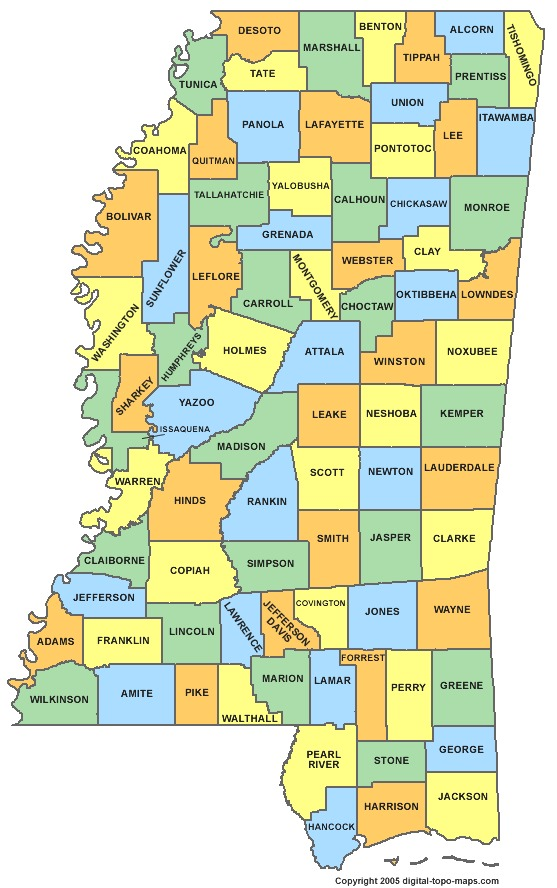
\includegraphics[width=.9\linewidth]{figures/county_map.jpg}
      \caption*{A Map of Counties in the State of Mississippi \cite{county_map}}
    \end{subfigure}~
    \begin{subfigure}[b]{0.5\textwidth}
      \center
      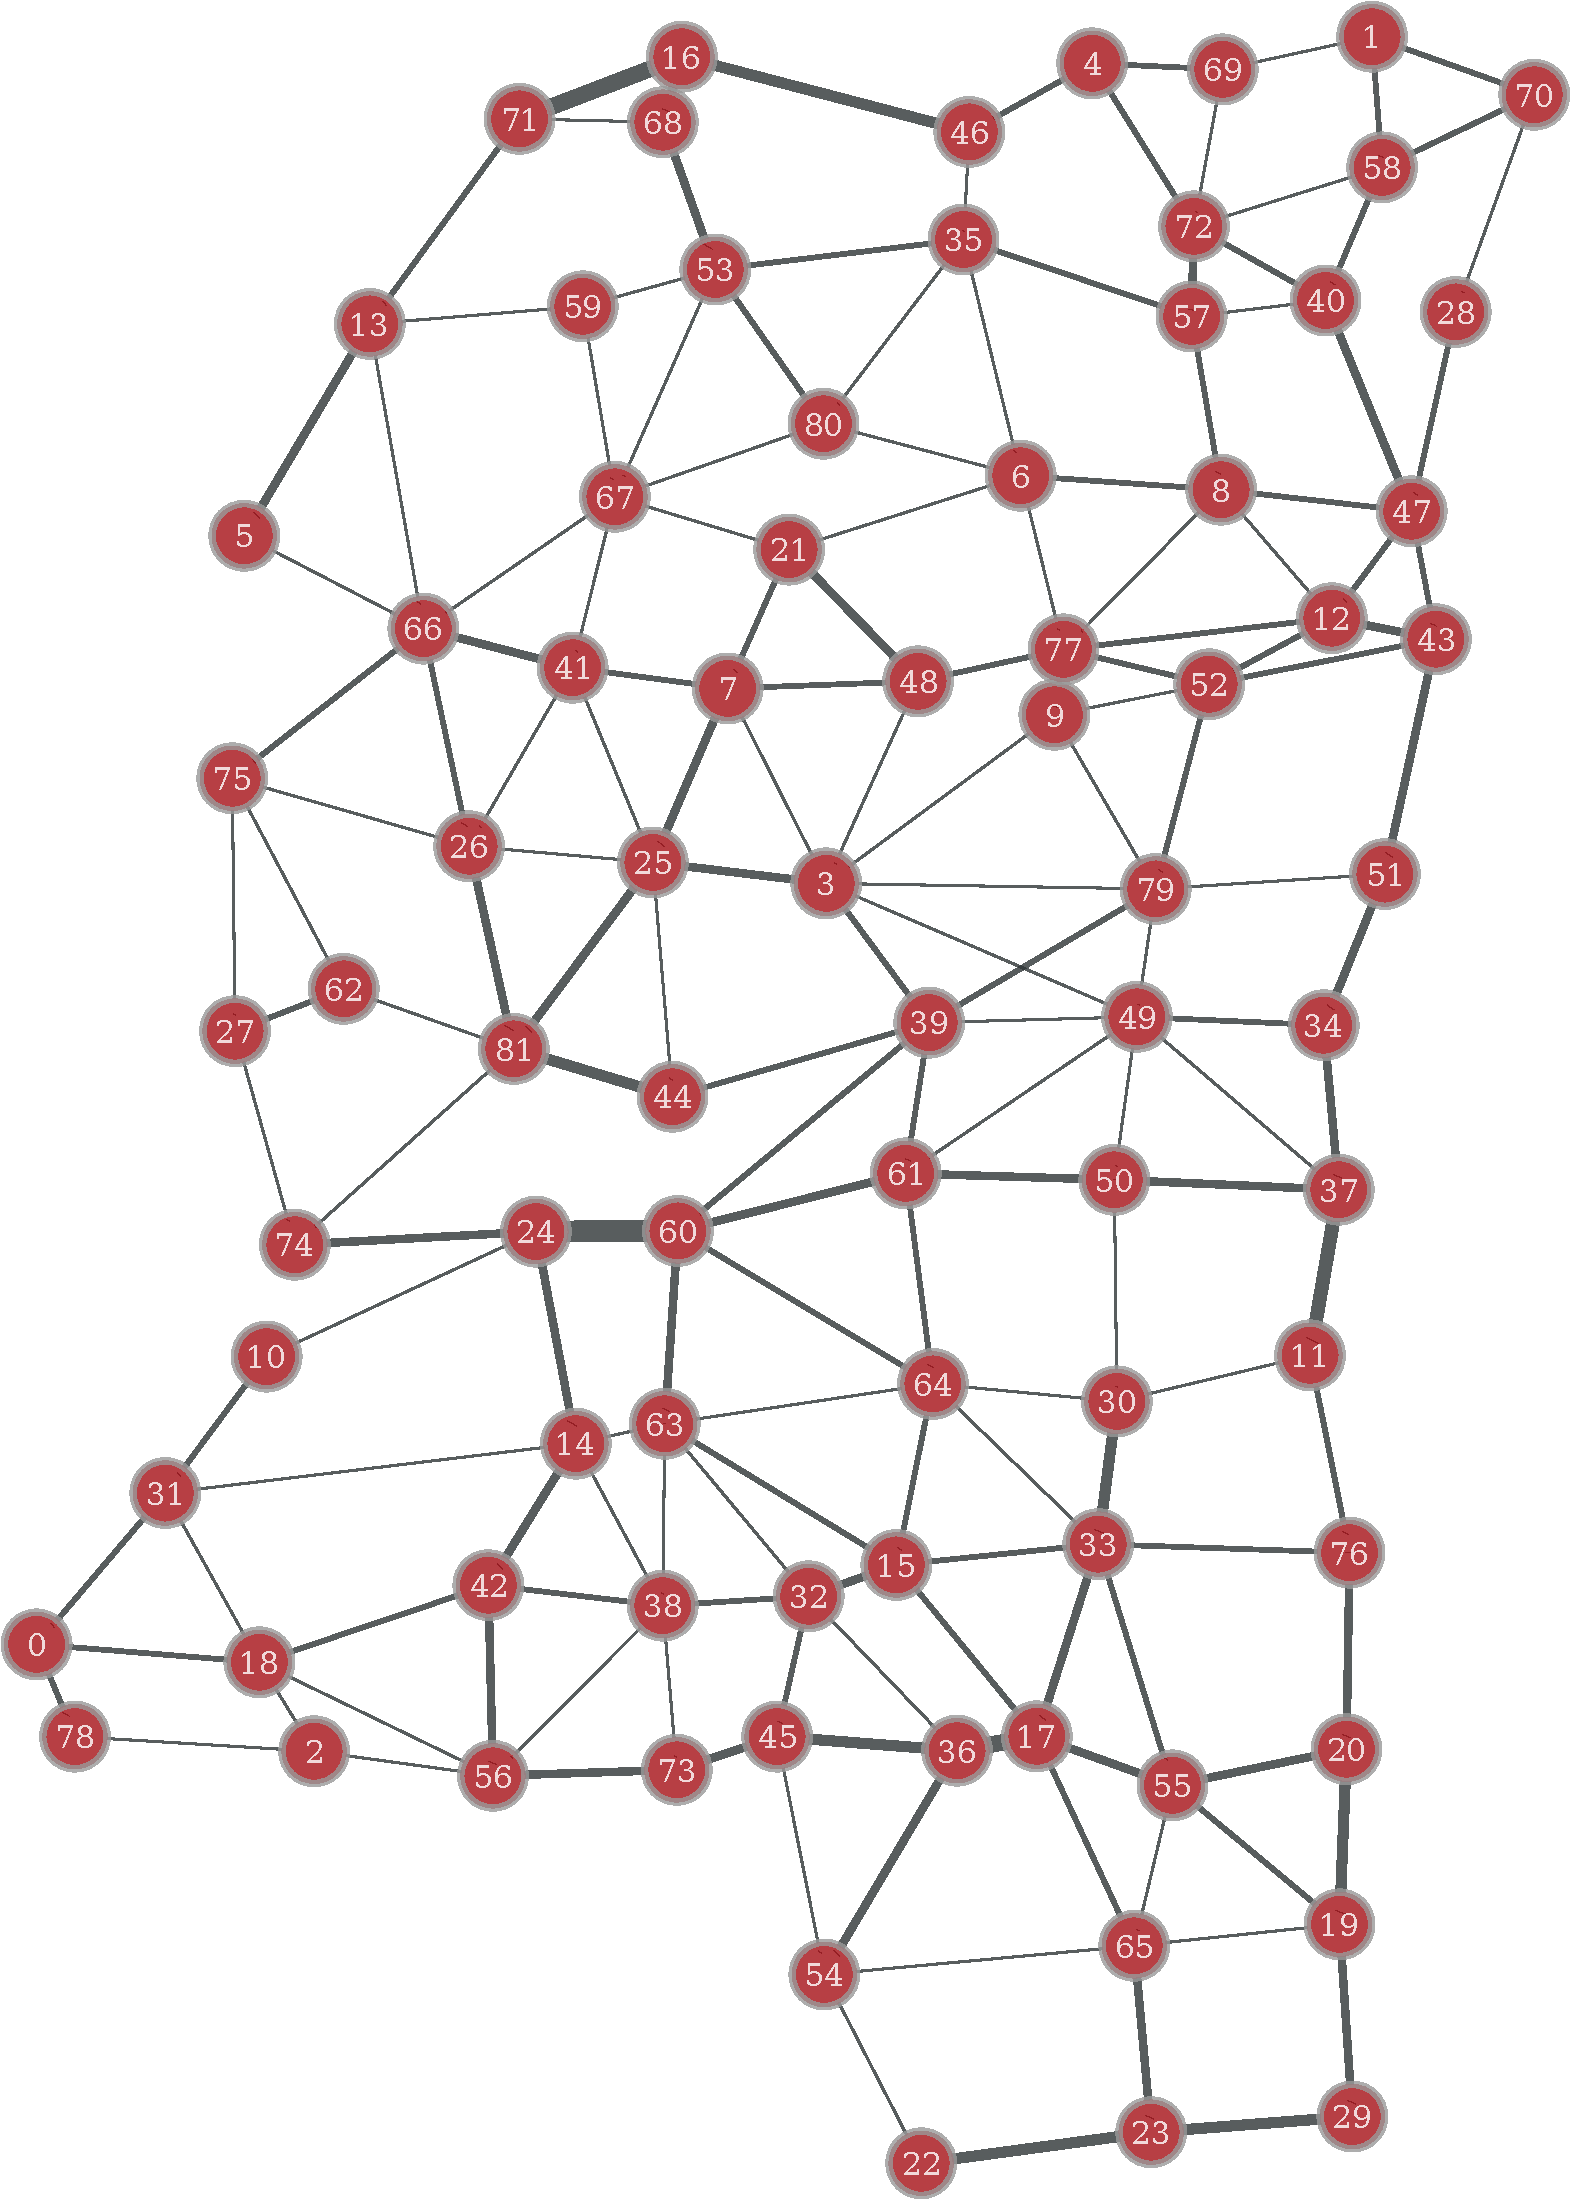
\includegraphics[width=\linewidth]{figures/full_undirected-crop.pdf}
      \caption*{Undirected Graph Representing Mississippi Counties}
    \end{subfigure}
    \caption*{}
  \end{figure}
  \par
     Because Mississippi has varying highway structure, it would be inappropriate to assume uniform travel rates between county pairs. In order to capture this heterogeneity in the network model, we decided to assign weights to every edge. Then a single edge weight represents a carrying capacity for the amount of travel possible between two counties. For a real-world mapping, we assume that this would correspond to the total number of highway lanes spanning two counties. Therefore, we were able to assign edge weights across the entire graph by using the following highway map:
  \begin{figure}[H]
    \centering
    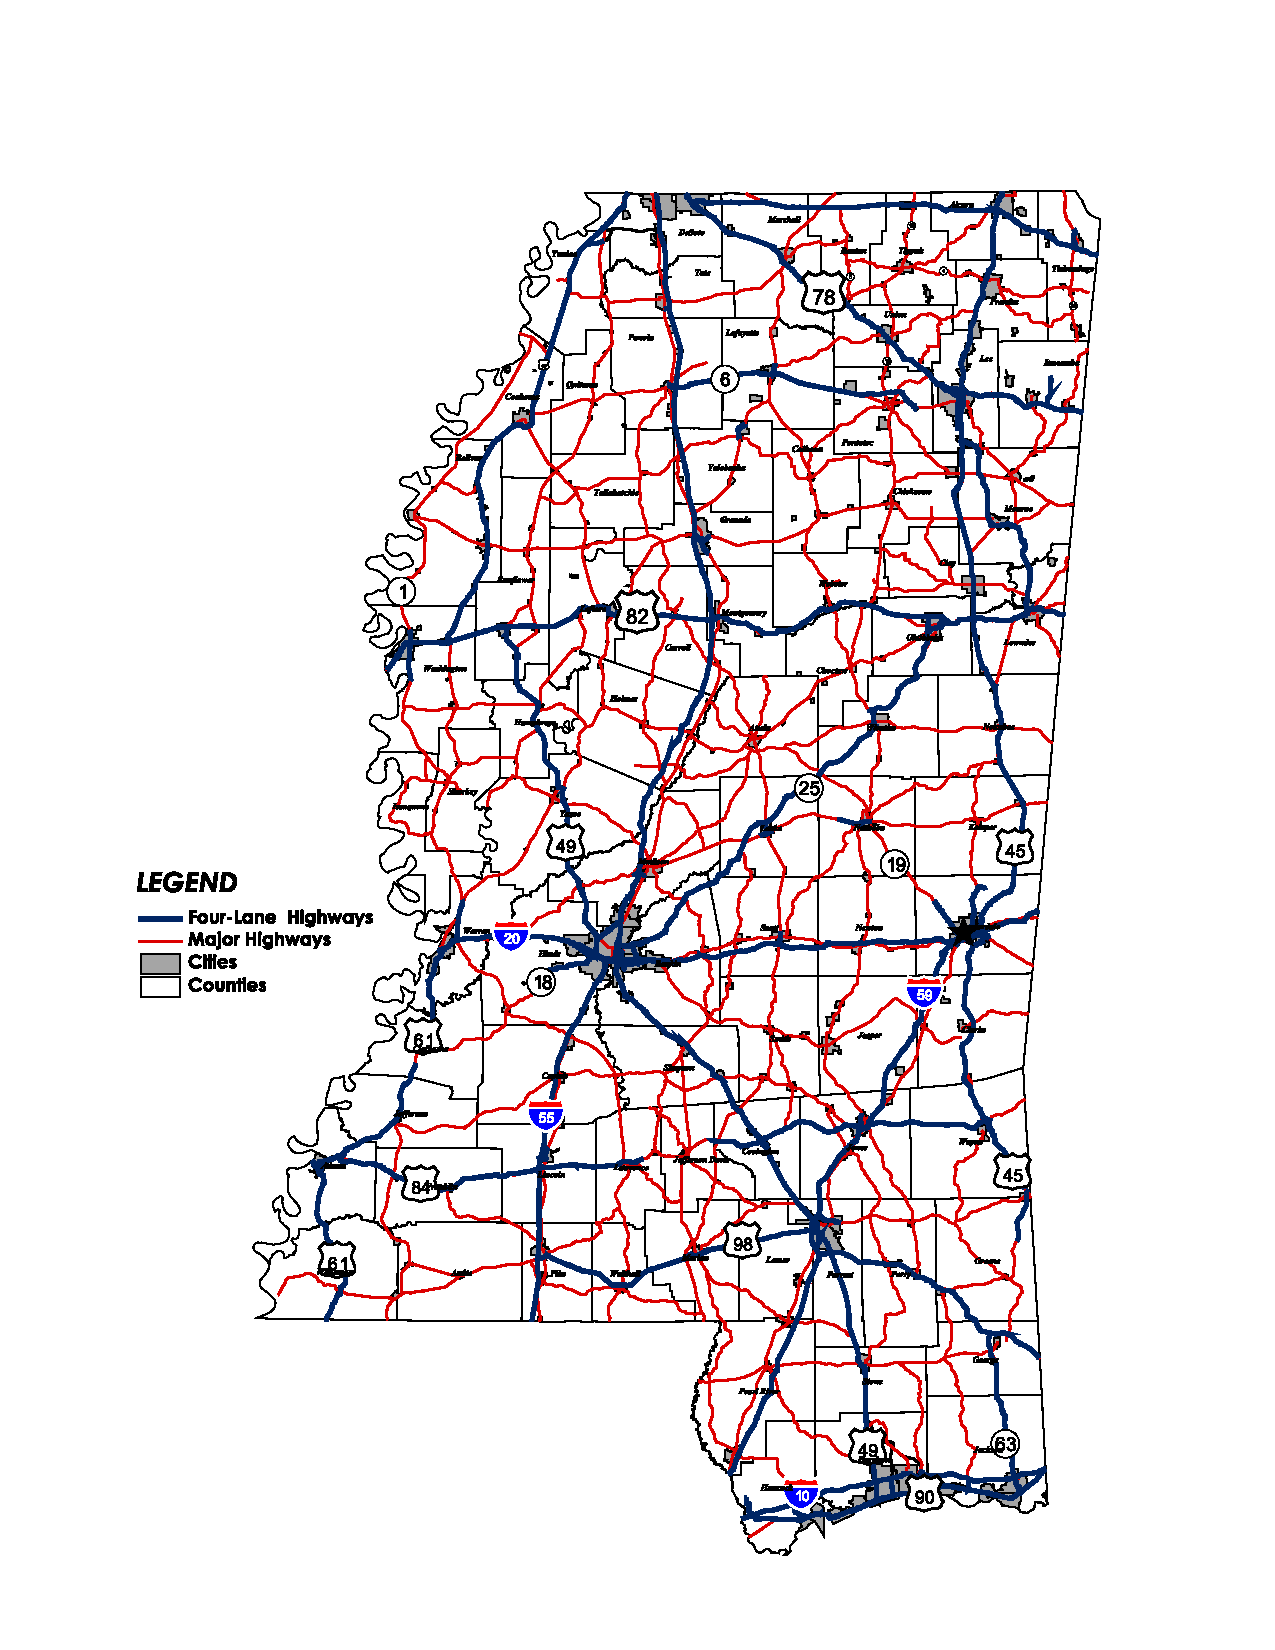
\includegraphics[width=.5\textwidth]{ms_highways.pdf}
    \caption{Map of Major Highways in the State of Mississippi \cite{ms_highways}}
    \label{fig:highway_map}
  \end{figure}
  \par
    In this figure, the thick black lines represent four lane highways while the red lines represent two lane highways. We assume that despite the ensuing panic, evacuees still travel along the right side of the highway, even if this means lanes going the other way (towards the hurricane) are underutilized. Therefore, for every thick black line spanning two counties, the appropriate edge in the graph gains two additional lanes, whereas red lines add one lane. Summing the lane contributions of all highways for a pair of counties therefore gives us an single edge weight in the graph.
  \newline
  \par
    We assume that there is a fixed spacing between every car on every highway. Then all cars travel at the same speed, and the density of cars is uniform along the entire length of every highway. This determines a fixed flow rate per edge capacity, and allows us to compute the number of cars traveling to another county in a given time interval. Because of the inevitable traffic congestion during an evacuation, we set the fixed speed to a relatively slow $10$ km/hr. In a traffic jam situation like this, we expect a tight traffic density of one car every 10 meters. Therefore:
    \[
      \frac{10\ \text{km/hr}}{10\ \text{m/car}} = 1000\ \text{cars/hr}
    \]
  \par
    We assume that evacuees travel with friends and family in their cars. Because the average size of an American family is \texttildelow 3 persons \cite{famsize}, we conclude that 3000 people per hour can use a single lane to another county. Maximum population flow rates between each county are therefore three thousand times the corresponding edge weight.

\section{Historical Hurricane Trends}
\label{sec:hurricanes}
  \par
    Northwest


\section{Markov Process Analysis of Strictly Northern Evacuations}
\label{sec:markov}
  Because our analysis of historical hurricane trends concluded that the vast majority of landfalls occur in the three southern-most counties, the first evacuation strategy we tested was one where all evacuees move strictly northward.
  \subsection{Model Description}
    Given that we have a network structure and associated population flow rates, this problem lends itself well to a Markov process analysis. We can model our evacuation strategy by converting the network of Mississippi counties into a directed graph. For our northward evacuation, this means only drawing highway-based edges to destination nodes with higher latitudes:
    \begin{figure}[H]
      \centering
      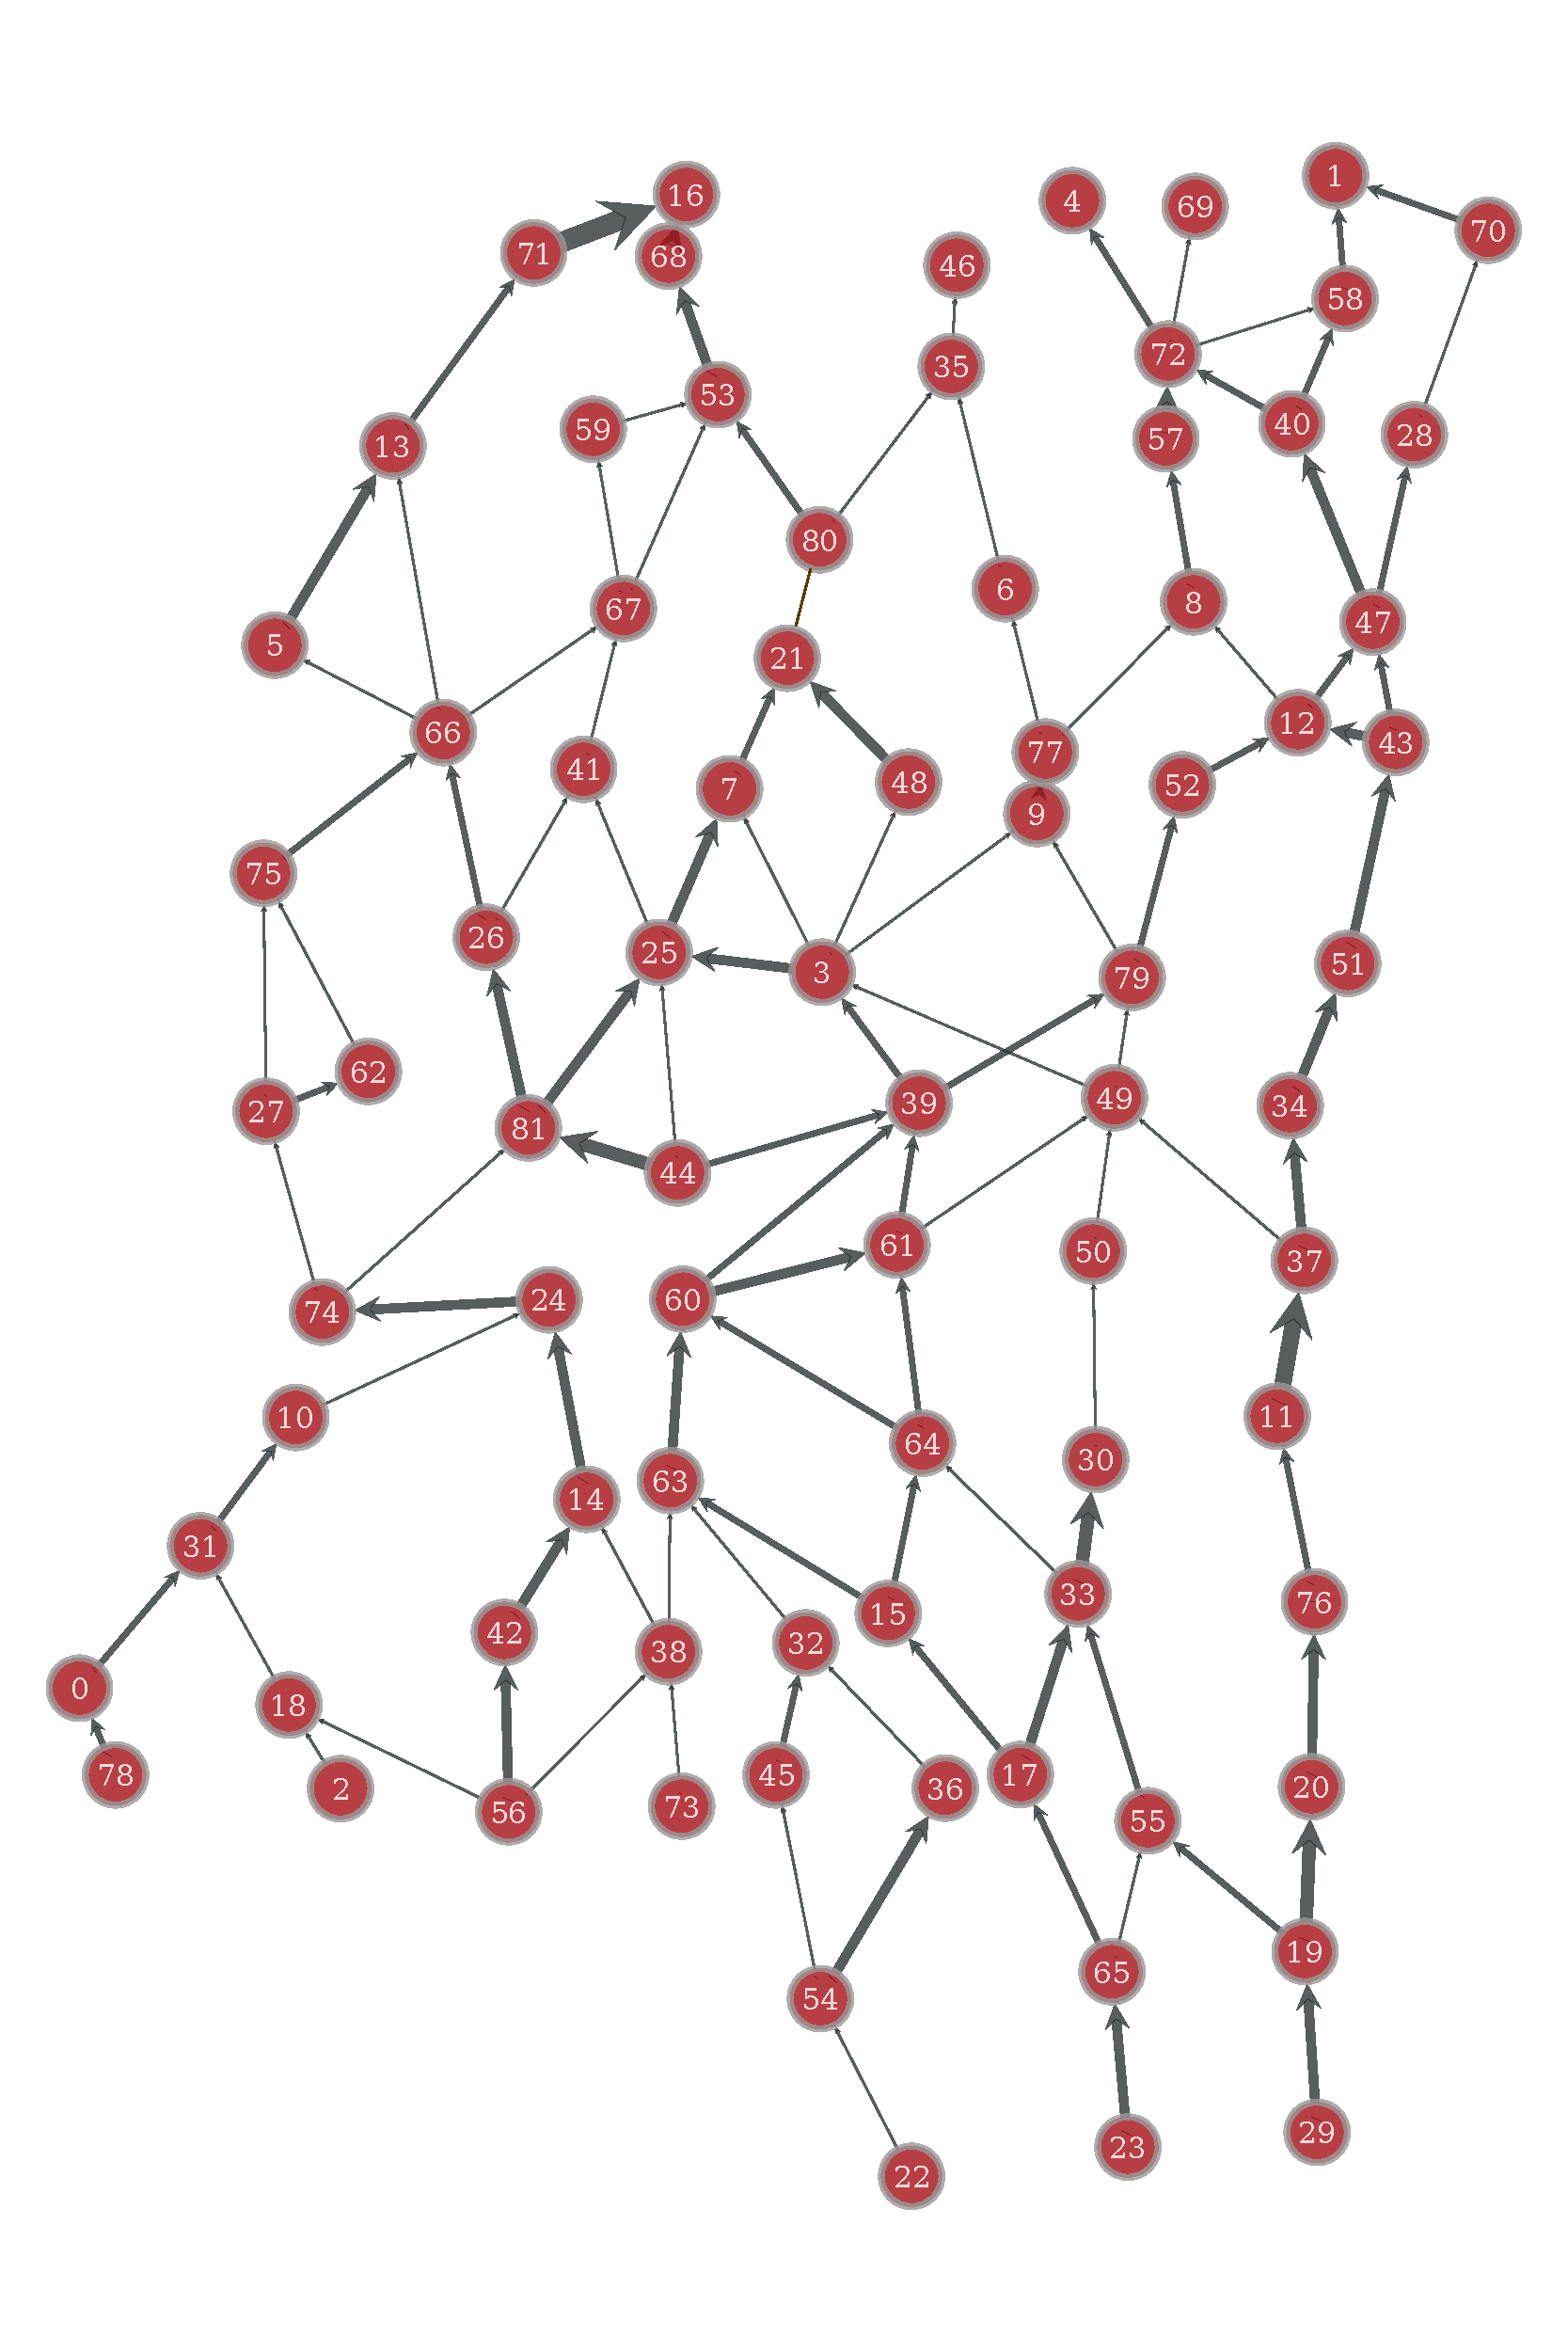
\includegraphics[width=.5\textwidth]{figures/full_directed_NS.pdf}
      \caption{Map of Northbound Highway Routes in the State of Mississippi \cite{ms_highways}}
    \end{figure}
    The thickness of each arrow in this graph represents the transition probability from one node to another. In evacuation terms, these are the proportions of a county's population that travel to a destination node during a single update. In order We standardize the time interval of an update to be one hour, and track the number of people in every county after each update in the 4 day period before landfall.

  \subsection{Parameter Values and Justification}
    Using our earlier values for the maximum flow rate of an edge, we can now use this 
  \subsection{Results}
  \subsection{Strengths and Weaknesses}

\section{Maximum Flow Analysis of Strictly Northern Evacuations}
\label{sec:maxflow}
  \subsection{Model Description}
    \par In this model, we will approach as a network flow problem. The nodes of this graph will be the counties, and the edges are the roads connecting them together. Since we also have a quantifiable way to compare roads based on their potential throughput, we can label those as the capacities of the edges.
    In order to get an idea of how many people can evacuate in a northbound manner, we can compute the maximum flow of the network. The location of the dividing line between the two partitions will also tell us the areas sof congestions, which will lead us to interesting plans.
  \subsection{Parameter Values and Justification}
    \par Now, in order to be able to compute the flow through the graph, we have to make it directed, and come up with a general rule for which directions we want to consider. After a lot of research, we saw that more often than not, going northbound was the best reaction to most hurricanes in Mississippi (because most of the hurricanes made landfall on the south coast).
    We also add two nodes to that graph that will act as the source and the sink (which are necessary for computing the maximum flow through the graph).
    \par It is worth noting that we did not consider the interactions with the other states as that would require knowing a lot more things about the highway systems and tendencies of the evacuees in those states. We also assumed that the counties that would need to be evacuated are the ones on the southern border of Mississippi; we will call them the evacuated counties.
  \subsection{Results}
  \par We computeed the max flow using a min-cut algorithm that was implemented as part of the Python \texttt{graph-tool} library \cite{graphtool}. Since the units of road are all integers, we expected an integer as the maximum flow through the graph (South to North), and that value turned out to be 21000 people moving in that direction per hour. The partitions are shown in red and blue in Figure~\ref{fig:oldmaxflow}.
  \par The interesting part, though, is that this information tells us where the bottleneck is in terms of transportation. By inspection, we can see that a new road linking counties 20 and 56 (George to Perry, located on the south east corner of the state) could increase the maximum flow number, as well as push the congestion areas further north (which means people can get further away from the hurricanes faster). 
  Indeed, after making this change, the max flow increased by over 25\% to 27000, and the partitions split much further north than before the addition of that road. Figure~\ref{fig:newmaxflow}
    \begin{figure}
      \center
      \begin{subfigure}[b]{0.5\textwidth}
        \center
        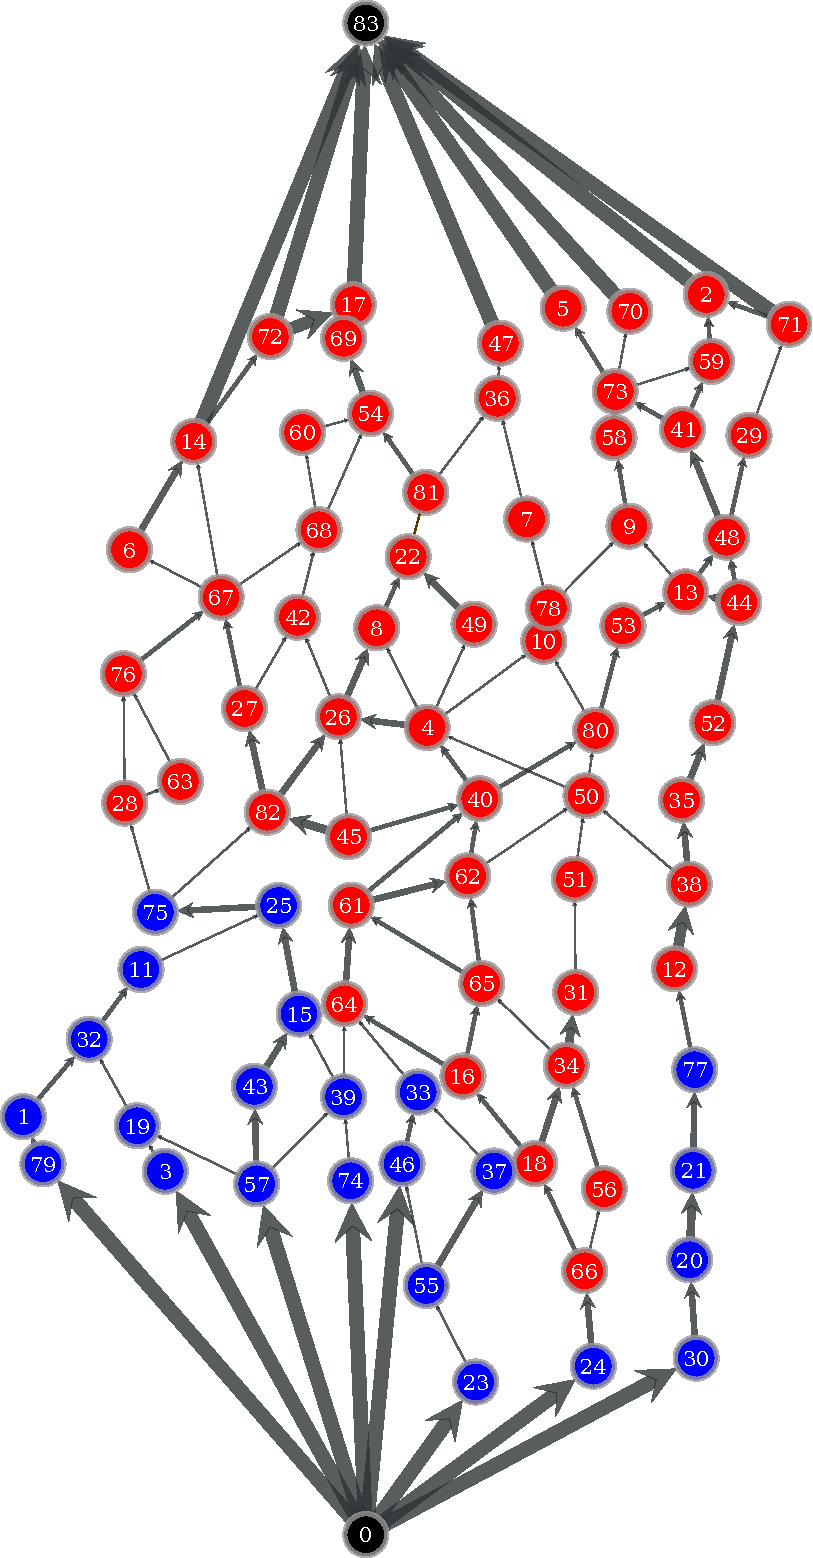
\includegraphics[width=\textwidth]{figures/old_maxflow-crop.pdf}
        \caption{Maximum Flow Partitions}
        \label{fig:oldmaxflow}
      \end{subfigure}~
      \begin{subfigure}[b]{0.5\textwidth}
        \center
        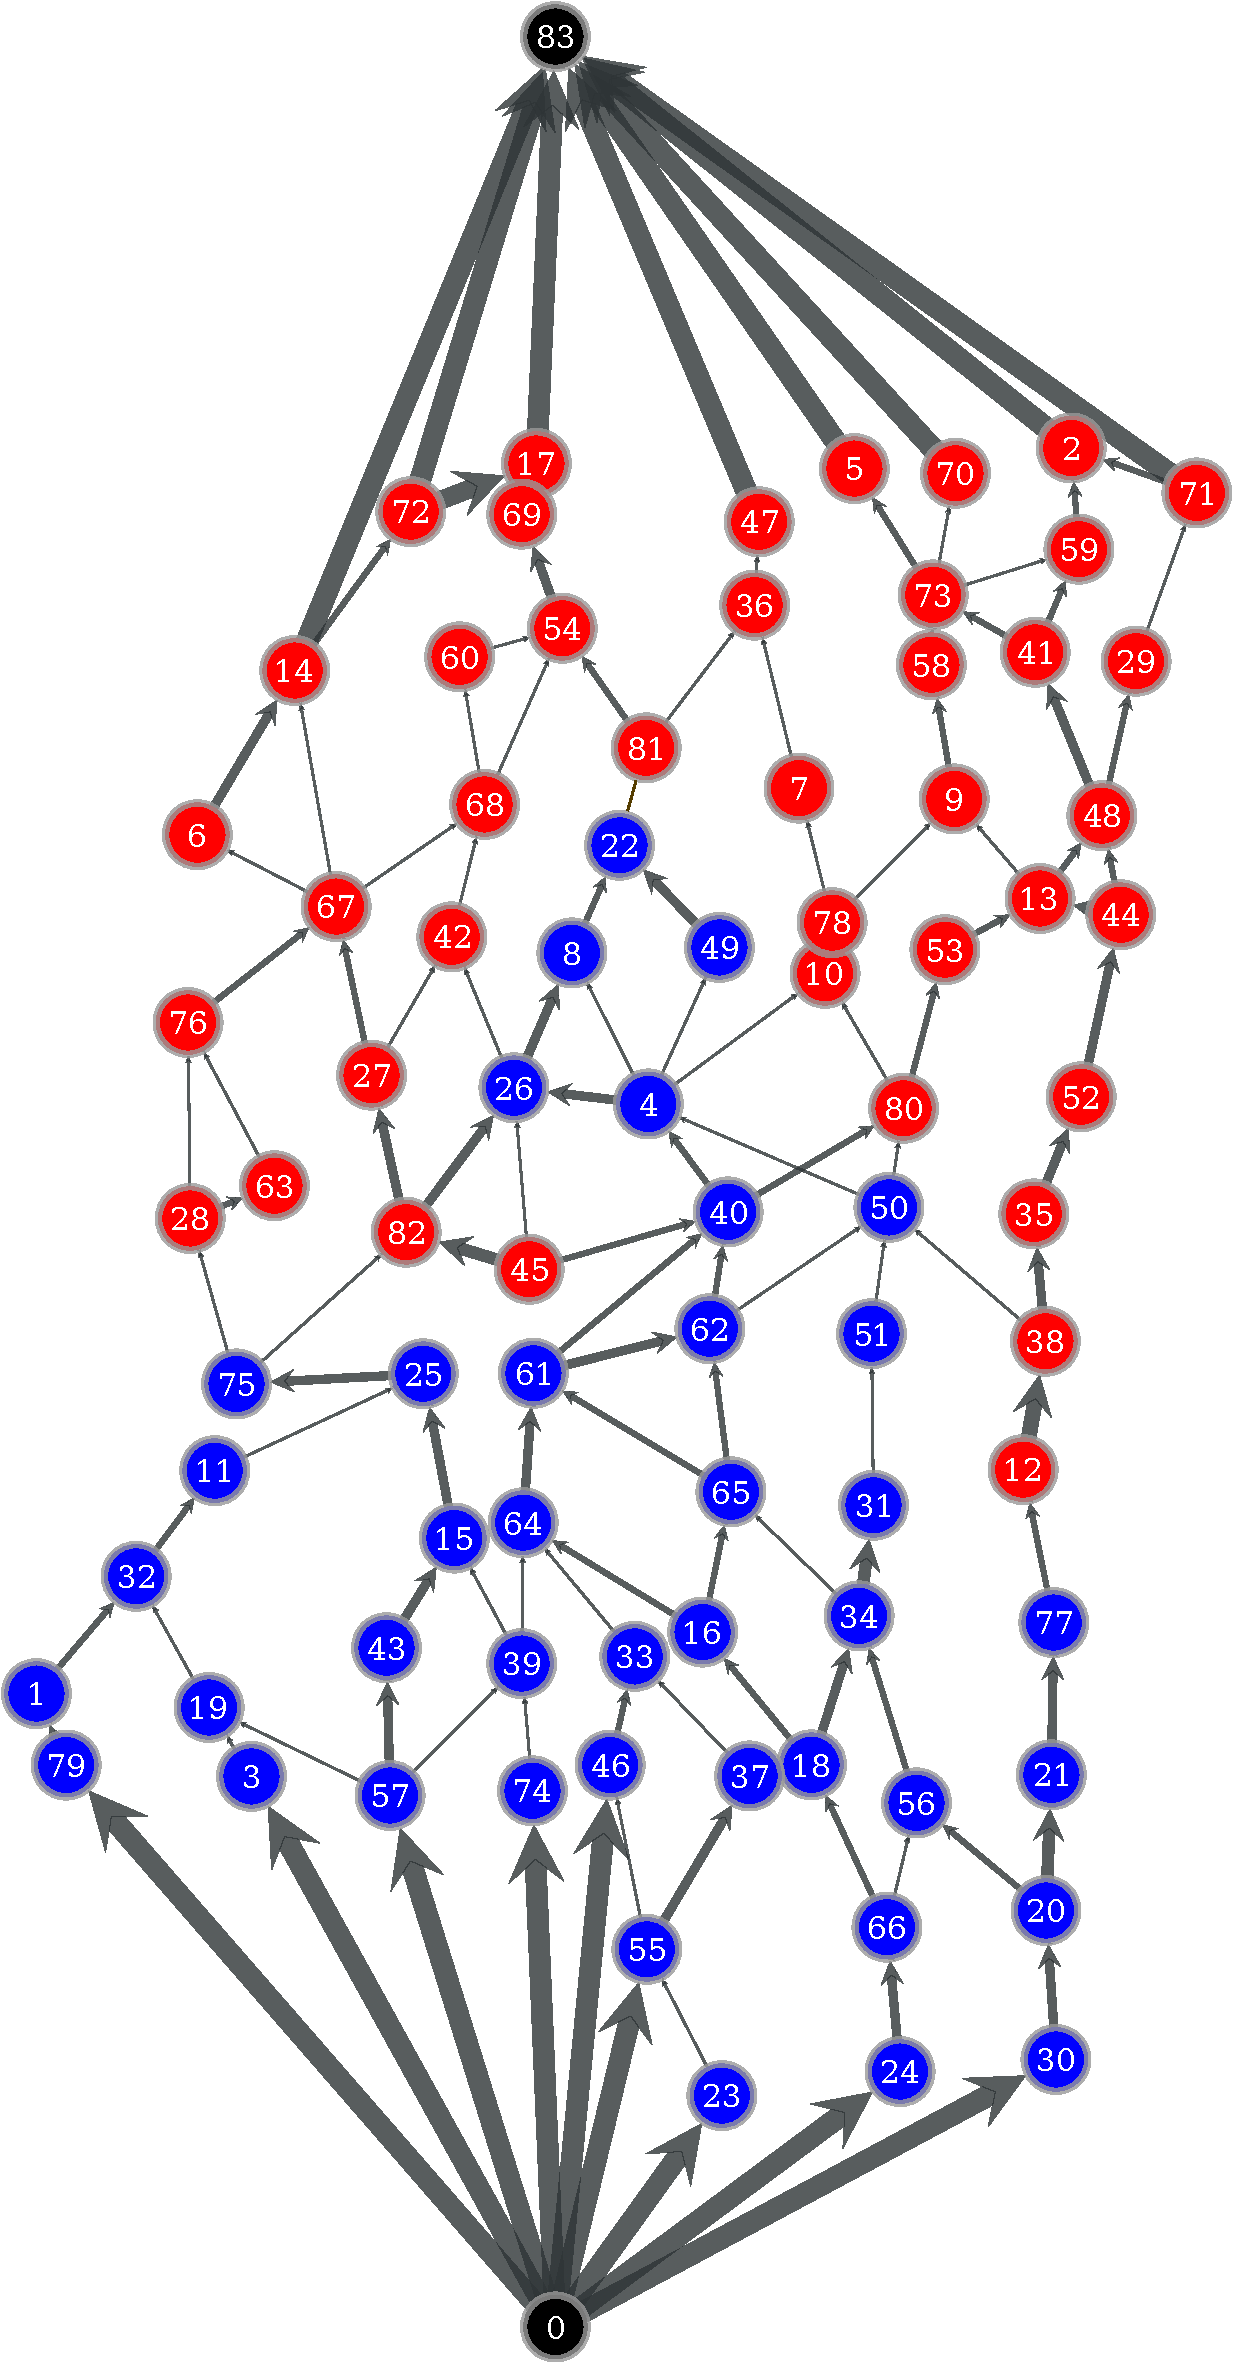
\includegraphics[width=\textwidth]{figures/maxflow_directed-crop.pdf}
        \caption{Maximum Flow Partitions}
        \label{fig:newmaxflow}
      \end{subfigure}
      \caption{}
    \end{figure}
    With this information, we can safely say that a great emergency evacuation plan could be prepared years in advance by creating new routes that link counties together. With the addition of a single two lane highway, we drastically increased the potential rate of evacuation of the southern counties. However, we can also use the maximum flow to determine how long in advance we need to order the evacuation.
    The total population of the evacuated counties is 616338. So let us compute the theoretical lower bound for how long it would take to evacuate those states fully:
    \begin{align*}
        t^* &= \frac{\text{total population}}{\text{max flow}}\\
        t^* &= \frac{532480}{21000}\\
        t^* &= 25 \text{hrs}
    \end{align*}
    So according to this model, if we decided to evacuate everyone in the southern counties all at once, it would take upwards of a day to get everyone to safe counties.
  \subsection{Strengths and Weaknesses}
    % TODO
    This model gives us a piece of information that no other model really touches: the roads that create a bottleneck in the evacuation. 

\section{Stochastic Model of Landfall-Avodiant Evacuations}
\label{sec:stochastic}
  \subsection{Model Description}
    \par In this model, instead of giving citizens particular evacuation plan, we give them a simple rule: move directly away from the hurricane landfall if possible, else move North or North-West. Using the statewide broadcast system, the state of Mississippi can tell its citizens where the expected landfall will be, and which counties will be the most affected. In which case, individual citizens are instructed to leave the counties that will be flooded, and to do so as outlined above. This means less coordination from the state, and more options for each citizens. At the cost of not having designated areas, and therefore designated refuge areas for citizens, evacuation is faster because it involves less per-county organization.\\
    \par As opposed to the model described in \nameref{sec:maxflow}, we also allow citizens to leave the state of Mississippi. For example, Arkansas is less likely to be hit by the full force of hurricanes that move through Mississippi \cite{5news}, as such, it is a good place to take refuge while the storm passes. In order to achieve this, we add ``unofficial'' nodes in the graph representation of Mississippi. Figure~\ref{fig:highway_map} shows that Hancock and Jackson Counties have roads that lead into Louisiana and Alabama respectively, both of which are potential routes away from the Hurricane's landfall, meaning that such nodes are important when movement can also be lateral. Because we are only interested in the movement of citizens within Mississippi, we can assume that citizens that reach the out-of-state nodes keep moving further and further away from the hurricane, though we are not tracking them. We created four out-of-state nodes North, South, East and West of Mississippi, each connected in a way that satisfies the highways mapped in Figure~\ref{fig:highway_map}.
  \subsection{Parameter Values and Justification}
    \par The parameters to this model are the same as the parameters for the models outlined above, except that this model uses the complete highway map of Mississippi, instead of only considering vertical highways. This algorithm expects three inputs outside of the parameters: the first, less accurate estimate of the affected counties, the more accurate second estimate and the final, most accurate estimate. Notice that as described, these inputs actually abstract away the hurricane's category. Instead, the category is reflected by the size of the list of the affected counties given as the respective inputs for the estimates. In order to generate these input, we used the historical hurricane data. Given the landfall and the hurricane's category, we can generate three sets of decreasing size containing neighboring counties. We can then run the simulation on these inputs.
  \subsection{Results}
    This model's main goal is to find the amount of time it takes to evacuate the affected states.
    \begin{figure}
      \center
      \begin{subfigure}[b]{0.5\textwidth}
        \center
        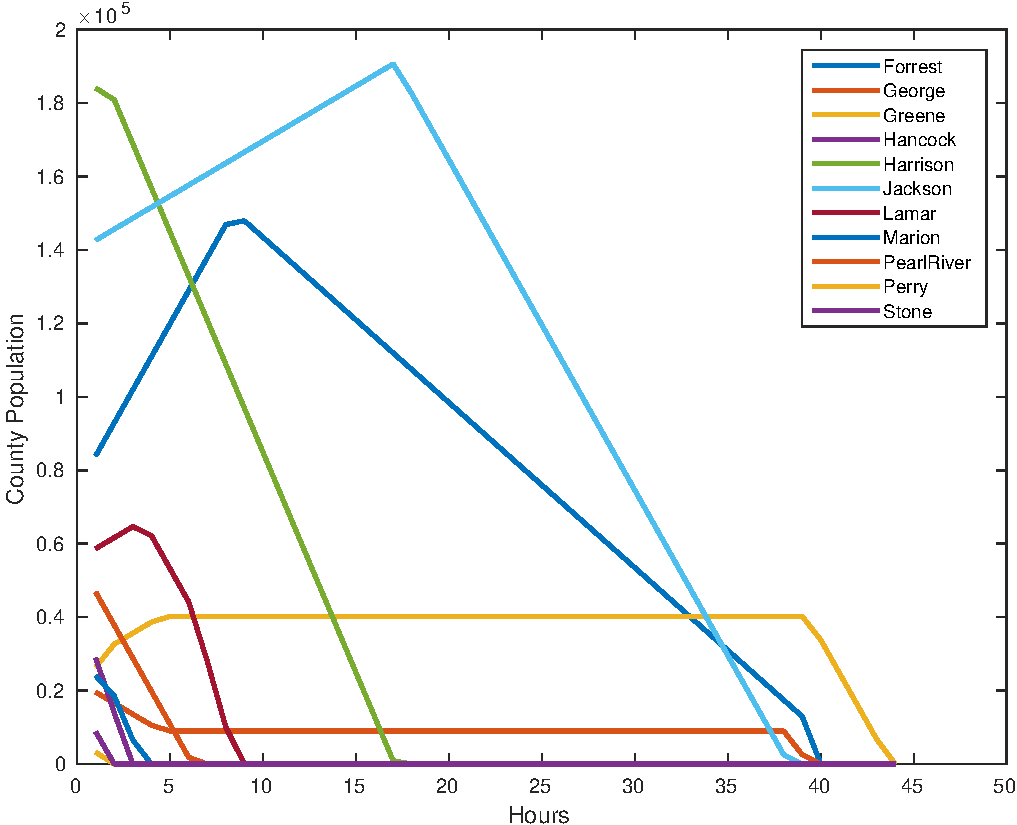
\includegraphics[width=\linewidth]{figures/pred_hancock-crop.pdf}
        \caption{Predicted Evacuation for Landfall in Hancock County}
      \end{subfigure}~
      \begin{subfigure}[b]{0.5\textwidth}
        \center
        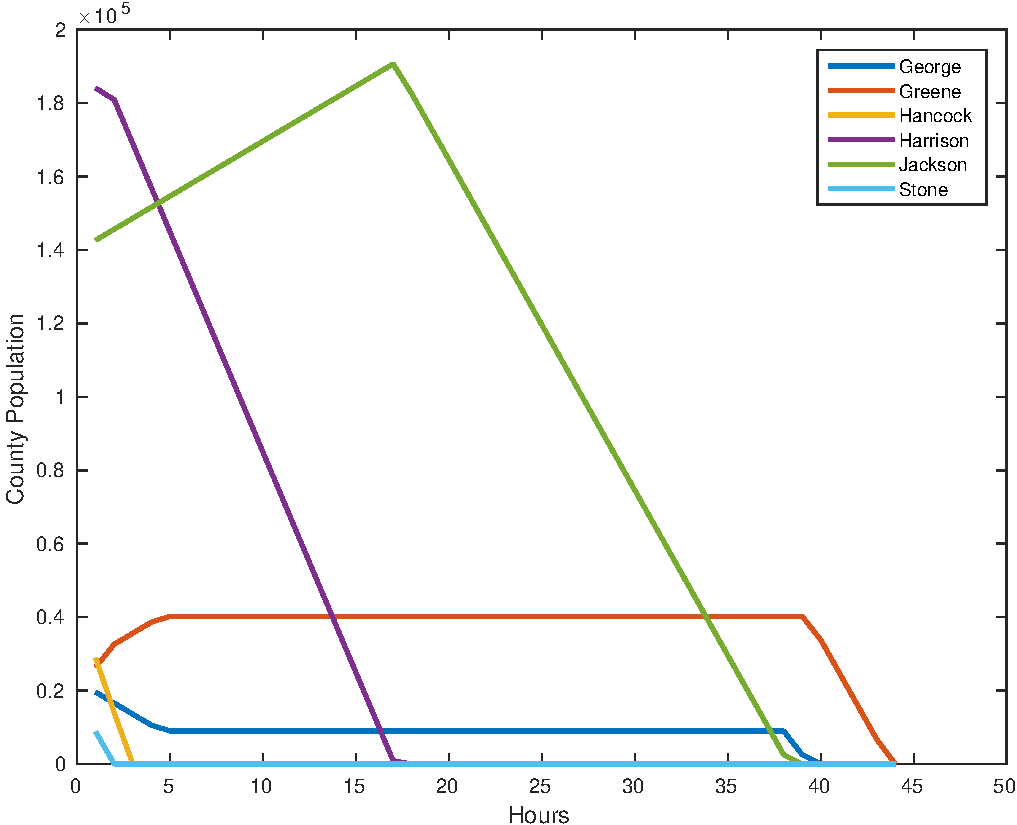
\includegraphics[width=\linewidth]{figures/pred_jackson-crop.pdf}
        \caption{Predicted Evacuation for Landfall in Jackson County}
      \end{subfigure}
      \caption{}
      \label{}
    \end{figure}
  \subsection{Strengths and Weaknesses}

\section{Conclusions}
\label{sec:conclusions}

\section{Future Work}
\label{sec:future}

\section{Individual Contributions}
\label{sec:contributions}
  \begin{thebibliography}{9}
    \bibitem{county_map}
      \url{http://www.madeinmississippi.us/wp-content/uploads/2015/02/mississippi-county-map.jpg}
    \bibitem{ms_highways}
      \url{https://www.mississippi.org/assets/docs/library/ms_highways.pdf}
    \bibitem{pmc}
      \url{http://www.ncbi.nlm.nih.gov/pmc/articles/PMC4060166/}
    \bibitem{5news}
      \url{http://5newsonline.com/2012/08/27/garretts-blog-hurricanes-in-arkansas/}
    \bibitem{famsize}
      \url{http://www.statista.com/statistics/183657/average-size-of-a-family-in-the-us/}
    \bibitem{graphtool}
      \url{http://graph-tool.skewed.de/}
    \bibitem{census}
      \url{http://census.ire.org/data/bulkdata.html}
  \end{thebibliography}

\lstinputlisting[style=Matlab]{deterministic/certainties.m}
\lstinputlisting[style=Matlab]{deterministic/constantrate.m}
\lstinputlisting[style=Matlab]{deterministic/getA.m}
\lstinputlisting[style=Matlab]{deterministic/populations.m}
\lstinputlisting[style=Matlab]{deterministic/thresholds.m}
\lstinputlisting[style=Matlab]{hurricane_generator/interpolate_radius.m}
\lstinputlisting[style=Python]{deterministic/threshold.py}
\lstinputlisting[style=Python]{get_pop.py}
\lstinputlisting[style=Python]{stochastic/data.py}
\lstinputlisting[style=Python]{stochastic/simulation.py}
\lstinputlisting[style=Python]{stochastic/wolfram.py}
\lstinputlisting[style=Python]{get_adjacency.py}
\lstinputlisting[style=Python]{utils.py}
\lstinputlisting[style=Python]{hurricane_generator/clean.py}
\lstinputlisting[style=Python]{hurricane_generator/get_radii.py}
\lstinputlisting[style=Python]{hurricane_generator/geotag.py}
\lstinputlisting[style=Python]{hurricane_generator/final.py}
\lstinputlisting[style=Python]{flow/colornodes.py}
\lstinputlisting[style=Python]{flow/maxflow.py}
\lstinputlisting[style=Python]{flow/create_graph.py}
\lstinputlisting[style=Python]{flow/threshold_from_hurricane.py}

\end{document}
